\documentclass[aspectratio=169,12pt]{beamer}

% =========================================================
% THEME
% =========================================================

\usetheme{Madrid}

% =========================================================
% PACKAGES
% =========================================================

\usepackage{amsmath}
\usepackage{amssymb}
\usepackage{booktabs}
\usepackage{array}
\usepackage{graphicx}
\usepackage{tikz}
\usepackage{xcolor}

\usetikzlibrary{
    arrows.meta,
    positioning,
    shapes.geometric,
    calc
}

% =========================================================
% PASTEL PROFESSIONAL COLORS
% =========================================================

\definecolor{PastelBlue}{RGB}{91,135,166}
\definecolor{PastelLavender}{RGB}{125,118,155}
\definecolor{LightBlue}{RGB}{235,242,247}
\definecolor{LightLavender}{RGB}{242,240,247}
\definecolor{DarkText}{RGB}{55,65,75}
\definecolor{PastelGreen}{RGB}{137,170,150}
\definecolor{LightGreen}{RGB}{237,245,239}

\setbeamercolor{structure}{fg=PastelBlue}

\setbeamercolor{normal text}{
    fg=DarkText,
    bg=white
}

\setbeamercolor{frametitle}{
    fg=PastelBlue,
    bg=LightBlue
}

\setbeamercolor{title}{
    fg=PastelBlue
}

\setbeamercolor{block title}{
    fg=white,
    bg=PastelBlue
}

\setbeamercolor{block body}{
    fg=DarkText,
    bg=LightBlue
}

\setbeamercolor{block title example}{
    fg=white,
    bg=PastelLavender
}

\setbeamercolor{block body example}{
    fg=DarkText,
    bg=LightLavender
}

\setbeamercolor{block title alerted}{
    fg=white,
    bg=PastelGreen
}

\setbeamercolor{block body alerted}{
    fg=DarkText,
    bg=LightGreen
}

% =========================================================
% FOOTER
% =========================================================

\setbeamertemplate{footline}
{
    \leavevmode%
    \hbox{%
        \begin{beamercolorbox}[
            wd=.33\paperwidth,
            ht=2.5ex,
            dp=1.125ex,
            leftskip=.3cm
        ]{author in head/foot}
            \usebeamerfont{author in head/foot}
            \insertshortauthor
        \end{beamercolorbox}%
        \begin{beamercolorbox}[
            wd=.34\paperwidth,
            ht=2.5ex,
            dp=1.125ex,
            center
        ]{title in head/foot}
            \usebeamerfont{title in head/foot}
            \insertshorttitle
        \end{beamercolorbox}%
        \begin{beamercolorbox}[
            wd=.33\paperwidth,
            ht=2.5ex,
            dp=1.125ex,
            rightskip=.3cm
        ]{date in head/foot}
            \usebeamerfont{date in head/foot}
            \hfill\insertshortdate\hspace{0.2cm}
        \end{beamercolorbox}%
    }%
    \vskip0pt%
}

\setbeamertemplate{navigation symbols}{}

% =========================================================
% DOCUMENT INFORMATION
% =========================================================

\title[N-Queens Using Predicate Calculus]
{N-Queens Problem Using Predicate Calculus}

\subtitle{
    Knowledge Representation and Constraint-Based Reasoning
}

\author[Arya T S]{Arya T S}

\institute{
    M.Tech Artificial Intelligence \& Software Engineering\\
    Cochin University of Science and Technology (CUSAT)
}

\date{October 2026}

% =========================================================
% DOCUMENT
% =========================================================

\begin{document}

% =========================================================
% TITLE SLIDE
% =========================================================

\begin{frame}[plain]
    \centering

    \vspace{0.8cm}

    {\usebeamerfont{title}
     \fontsize{27}{33}\selectfont
     \bfseries\color{PastelBlue}
     N-Queens Problem Using Predicate Calculus
     \par}

    \vspace{0.4cm}

    {\large\color{PastelLavender}
     Knowledge Representation and Constraint-Based Reasoning
     \par}

    \vspace{1.0cm}

    {\large\color{DarkText}
     Arya T S
     \par}

    \vspace{0.4cm}

    {\normalsize\color{DarkText}
     M.Tech Artificial Intelligence \& Software Engineering
     \par}

    {\normalsize\color{DarkText}
     Cochin University of Science and Technology (CUSAT)
     \par}

    \vspace{0.6cm}

    {\normalsize\color{DarkText}
     October 2026
     \par}

\end{frame}

% =========================================================
% MODULE OVERVIEW -- SLIDE 1
% =========================================================

\begin{frame}{Project Overview}

\begin{columns}[T,totalwidth=\textwidth]

\begin{column}{0.48\textwidth}

\begin{block}{Part I -- Foundations}

\begin{itemize}
    \item N-Queens Problem
    \item Problem Statement
    \item Objectives
    \item Predicate Calculus
    \item Knowledge Representation
\end{itemize}

\end{block}

\end{column}

\begin{column}{0.48\textwidth}

\begin{block}{Part II -- Implementation}

\begin{itemize}
    \item Logical Constraints
    \item Z3 Solver
    \item System Architecture
    \item AI and User Modes
    \item Testing and Validation
\end{itemize}

\end{block}

\end{column}

\end{columns}

\end{frame}

% =========================================================
% MODULE OVERVIEW -- SLIDE 2
% =========================================================

\begin{frame}{Project Overview}

\begin{columns}[T,totalwidth=\textwidth]

\begin{column}{0.48\textwidth}

\begin{block}{Part III -- Application Features}

\begin{itemize}
    \item Board Sizes from 1 to 13
    \item Interactive Chessboard
    \item AI-Based Solution
    \item Hint Generation
    \item Timer and Win Detection
    \item Light and Dark Themes
\end{itemize}

\end{block}

\end{column}

\begin{column}{0.48\textwidth}

\begin{block}{Part IV -- Evaluation}

\begin{itemize}
    \item Satisfiability Checking
    \item Solution Validation
    \item Unsatisfiable Cases
    \item Constraint-Based Reasoning
    \item Limitations
    \item Future Enhancements
\end{itemize}

\end{block}

\end{column}

\end{columns}

\end{frame}

% =========================================================
% SLIDE 3 -- INTRODUCTION
% =========================================================

\begin{frame}{Introduction}

\begin{block}{What is the N-Queens Problem?}

The N-Queens problem requires placing $N$ queens on an
$N \times N$ chessboard such that no two queens attack
each other.
\end{block}

\begin{columns}[T,totalwidth=\textwidth]

\begin{column}{0.48\textwidth}

\begin{block}{Core Constraints}

\begin{itemize}
    \item Exactly one queen in each row.
    \item No two queens share a column.
    \item No two queens share a diagonal.
\end{itemize}

\end{block}

\end{column}

\begin{column}{0.48\textwidth}

\begin{exampleblock}{AI Perspective}

The problem can be represented as a set of logical
constraints and solved by searching for an assignment
that satisfies all constraints.
\end{exampleblock}

\end{column}

\end{columns}

\end{frame}

% =========================================================
% SLIDE 4 -- PROBLEM STATEMENT
% =========================================================

\begin{frame}{Problem Statement}

\begin{block}{Problem Definition}

Given an integer $N$, determine a placement of $N$ queens
on an $N \times N$ chessboard such that every queen
satisfies the non-attacking constraints.
\end{block}

\textbf{Input:}
\begin{itemize}
    \item Board size $N$, where $1 \leq N \leq 13$.
    \item Optional fixed queen placements.
\end{itemize}

\textbf{Output:}
\begin{itemize}
    \item A valid board configuration, if one exists.
    \item An unsatisfiable result if no valid configuration
          exists under the given constraints.
\end{itemize}

\begin{alertblock}{Important Observation}

For the standard problem, solutions exist for $N=1$ and
all $N \geq 4$. No solution exists for $N=2$ or $N=3$.
\end{alertblock}

\end{frame}

% =========================================================
% SLIDE 5 -- OBJECTIVES
% =========================================================

\begin{frame}{Project Objectives}

\begin{enumerate}
    \item Represent the N-Queens problem using
          predicate-calculus concepts.
    \item Express row, column, and diagonal requirements
          as logical constraints.
    \item Encode the finite constraints using the Z3 solver.
    \item Generate valid solutions through satisfiability
          checking.
    \item Develop an interactive application for solving
          and playing the puzzle.
    \item Validate the solver using satisfiable and
          unsatisfiable test cases.
\end{enumerate}

\end{frame}

% =========================================================
% SLIDE 6 -- PREDICATE CALCULUS
% =========================================================

\begin{frame}{Predicate Calculus Representation}
\vspace{-0.3cm}
\begin{block}{Predicate Definition}

Let $Q(r,c)$ denote:

\[
Q(r,c) =
\begin{cases}
\text{True}, & \text{if a queen occupies }(r,c),\\
\text{False}, & \text{otherwise}.
\end{cases}
\]

The variables $r$ and $c$ represent row and column indices.
\end{block}

\begin{exampleblock}{Finite Domain}

\[
r,c \in \{0,1,\ldots,N-1\}
\]

The board is represented as a finite domain over which
the logical constraints are instantiated.
\end{exampleblock}

\textbf{Goal:} Find an assignment to the predicates that
satisfies every constraint.

\end{frame}

% =========================================================
% SLIDE 7 -- ROW CONSTRAINTS
% =========================================================

\begin{frame}{Logical Constraint I -- Row Uniqueness}
\vspace{-0.3cm}
Every row must contain exactly one queen.

\begin{block}{At Least One Queen in Every Row}

\[
\forall r\ \exists c\ Q(r,c)
\]

This ensures that every row contains a queen.
\end{block}

\begin{block}{At Most One Queen in Every Row}

\[
\begin{aligned}
\forall r,c_1,c_2,\quad
&\big(Q(r,c_1)\land Q(r,c_2)\big)\\
&\Rightarrow c_1=c_2
\end{aligned}
\]

This prevents multiple queens from occupying the same row.
\end{block}

\begin{exampleblock}{Combined Requirement}

Every row contains exactly one queen.
\end{exampleblock}

\end{frame}

% =========================================================
% SLIDE 8 -- COLUMN CONSTRAINTS
% =========================================================

\begin{frame}{Logical Constraint II -- Column Uniqueness}

No two queens may occupy the same column.

\begin{block}{Predicate-Calculus Formula}

\[
\begin{aligned}
\forall r_1,r_2,c,\quad
&\big(Q(r_1,c)\land Q(r_2,c)\big)\\
&\Rightarrow r_1=r_2
\end{aligned}
\]

\end{block}

\begin{columns}[T,totalwidth=\textwidth]

\begin{column}{0.48\textwidth}

\begin{exampleblock}{Valid Placement}

Queens occupy different columns.
\end{exampleblock}

\end{column}

\begin{column}{0.48\textwidth}

\begin{alertblock}{Invalid Placement}

Two queens in the same column violate the constraint.
\end{alertblock}

\end{column}

\end{columns}

\textbf{Purpose:} Eliminate board configurations containing
a vertical attack.

\end{frame}

% =========================================================
% SLIDE 9 -- DIAGONAL CONSTRAINTS
% =========================================================

\begin{frame}{Logical Constraint III -- Diagonal Safety}

Two queens attack each other diagonally when the absolute
difference between their row indices equals the absolute
difference between their column indices.

\begin{block}{Predicate-Calculus Formula}

\[
\begin{aligned}
\forall r_1,r_2,c_1,c_2,\quad
&\big(Q(r_1,c_1)\land Q(r_2,c_2)\\
&\land r_1\ne r_2\big)\\
&\Rightarrow |r_1-r_2|\ne |c_1-c_2|
\end{aligned}
\]

\end{block}

\begin{exampleblock}{Interpretation}

If two queens are in different rows, their row and column
differences must not be equal in magnitude.
\end{exampleblock}

\end{frame}

% =========================================================
% SLIDE 10 -- COMBINED LOGICAL MODEL
% =========================================================

\begin{frame}{Combined Logical Model}

The solution must satisfy all the following requirements.

\begin{enumerate}
    \item \textbf{Row constraint:} Exactly one queen in
          every row.
    \item \textbf{Column constraint:} No two queens in
          the same column.
    \item \textbf{Diagonal constraint:} No two queens
          on the same diagonal.
    \item \textbf{Fixed-position constraint:} Any queen
          specified by the user must remain in its
          designated square.
\end{enumerate}

\begin{block}{Satisfiability}

Let $C$ denote the conjunction of all constraints.

\[
C = C_{\text{row}}\land C_{\text{column}}
    \land C_{\text{diagonal}}\land C_{\text{fixed}}
\]

The solver searches for an assignment satisfying $C$.
\end{block}

\end{frame}

% =========================================================
% SLIDE 11 -- Z3 SOLVER
% =========================================================

\begin{frame}{Z3 Constraint Solver}
\vspace{-0.3cm}
\begin{block}{What is Z3?}

Z3 is an SMT (Satisfiability Modulo Theories) solver that
determines whether a set of logical constraints can be
satisfied and can produce a satisfying model.
\end{block}
\vspace{-0.3cm}
\begin{columns}[T,totalwidth=\textwidth]

\begin{column}{0.48\textwidth}
\vspace{-0.3cm}
\begin{block}{In This Project}

\begin{itemize}
    \item Boolean variables represent board squares.
    \item Row constraints use pseudo-Boolean equality.
    \item Column and diagonal constraints prohibit
          conflicting queen placements.
    \item Fixed queens become additional constraints.
\end{itemize}

\end{block}

\end{column}

\begin{column}{0.48\textwidth}

\begin{exampleblock}{Solver Results}

\begin{itemize}
    \item \texttt{sat}: a valid assignment exists.
    \item \texttt{unsat}: constraints cannot be satisfied.
    \item A satisfying model identifies queen positions.
\end{itemize}

\end{exampleblock}

\end{column}

\end{columns}

\end{frame}

% =========================================================
% SLIDE 12 -- LOGIC TO IMPLEMENTATION
% =========================================================

\begin{frame}{From Predicate Calculus to Z3}

\begin{center}

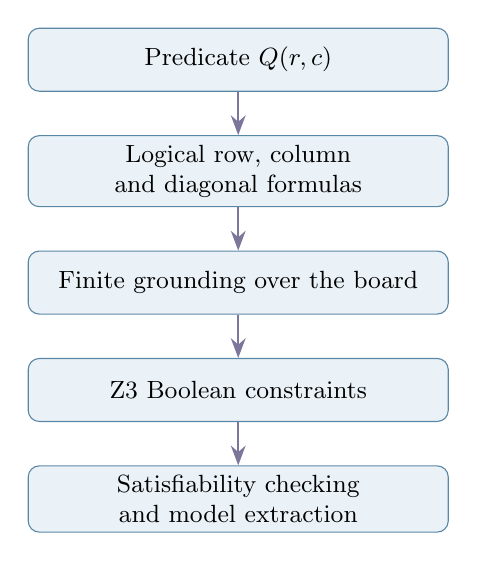
\begin{tikzpicture}[
    node distance=0.55cm,
    every node/.style={font=\small},
    process/.style={
        rectangle,
        rounded corners,
        draw=PastelBlue,
        fill=LightBlue,
        text width=5.1cm,
        minimum height=0.8cm,
        align=center
    },
    arrow/.style={
        -{Stealth[length=2.5mm]},
        thick,
        draw=PastelLavender
    }
]

\node[process] (p) {Predicate $Q(r,c)$};

\node[process, below=of p] (f) {Logical row, column and diagonal formulas};

\node[process, below=of f] (g) {Finite grounding over the board};

\node[process, below=of g] (z) {Z3 Boolean constraints};

\node[process, below=of z] (s) {Satisfiability checking and model extraction};

\draw[arrow] (p) -- (f);
\draw[arrow] (f) -- (g);
\draw[arrow] (g) -- (z);
\draw[arrow] (z) -- (s);

\end{tikzpicture}

\end{center}

\end{frame}

% =========================================================
% SLIDE 13 -- SYSTEM ARCHITECTURE
% =========================================================

\begin{frame}{System Architecture}

\begin{center}

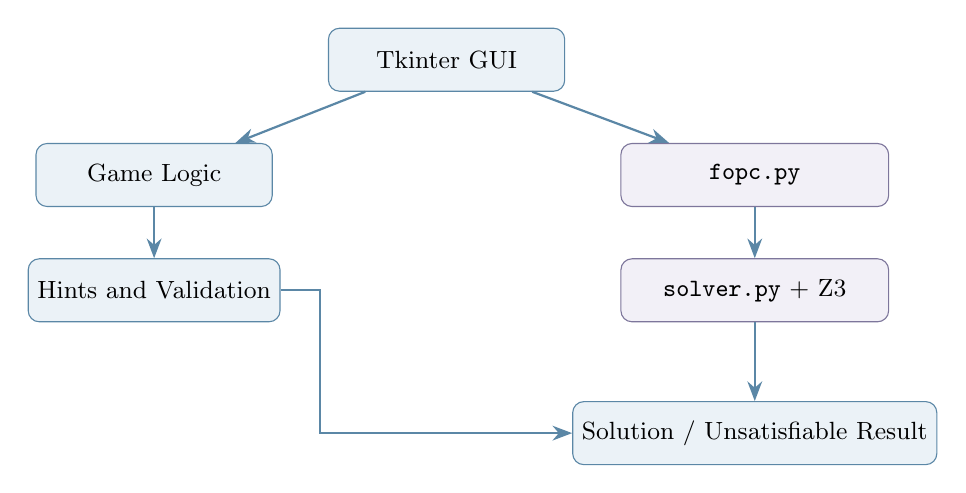
\begin{tikzpicture}[
    node distance=0.65cm and 0.7cm,
    every node/.style={font=\small},
    module/.style={
        rectangle,
        rounded corners,
        draw=PastelBlue,
        fill=LightBlue,
        minimum width=3.0cm,
        minimum height=0.8cm,
        align=center
    },
    logic/.style={
        rectangle,
        rounded corners,
        draw=PastelLavender,
        fill=LightLavender,
        minimum width=3.4cm,
        minimum height=0.8cm,
        align=center
    },
    arrow/.style={
        -{Stealth[length=2.5mm]},
        thick,
        draw=PastelBlue
    }
]

\node[module] (ui) {Tkinter GUI};

\node[module, below left=of ui] (game) {Game Logic};

\node[logic, below right=of ui] (fopc) {\texttt{fopc.py}};

\node[logic, below=of fopc] (solver) {\texttt{solver.py} + Z3};

\node[module, below=of game] (hint) {Hints and Validation};

\node[module, below=1.0cm of solver] (result) {Solution / Unsatisfiable Result};

\draw[arrow] (ui) -- (game);
\draw[arrow] (ui) -- (fopc);
\draw[arrow] (game) -- (hint);
\draw[arrow] (fopc) -- (solver);
\draw[arrow] (solver) -- (result);
\draw[arrow] (hint.east) -- ++(0.5,0) |- (result.west);

\end{tikzpicture}

\end{center}

\vspace{0.2cm}

\centering
\small The GUI handles interaction, while the logical model
and Z3 solver handle constraint-based reasoning.

\end{frame}

% =========================================================
% SLIDE 14 -- WORKFLOW
% =========================================================

\begin{frame}{Application Workflow}

\begin{enumerate}
    \item Select the board size.
    \item Choose AI mode or user mode.
    \item Generate logical constraints for the board.
    \item Ask Z3 to find a satisfying assignment when an
          AI solution is requested.
    \item Display the resulting queen positions.
    \item In user mode, validate each move against the
          non-attacking rules.
    \item Detect a completed valid board and display
          the win message.
\end{enumerate}

\begin{block}{Hint Mechanism}

A hint can be generated by asking the solver for a valid
completion consistent with the current queen placements.
\end{block}

\end{frame}

% =========================================================
% SLIDE 15 -- APPLICATION FEATURES
% =========================================================

\begin{frame}{Application Features}

\begin{columns}[T,totalwidth=\textwidth]

\begin{column}{0.48\textwidth}

\begin{block}{Solving Features}

\begin{itemize}
    \item Board size from 1 to 13.
    \item AI solution generation.
    \item User-controlled queen placement.
    \item Constraint-based move validation.
    \item Hint generation.
\end{itemize}

\end{block}

\end{column}

\begin{column}{0.48\textwidth}

\begin{block}{Interface Features}

\begin{itemize}
    \item Interactive chessboard.
    \item Light and dark themes.
    \item Game timer.
    \item Win detection and feedback.
    \item Fixed queen placements, where supported.
\end{itemize}

\end{block}

\end{column}

\end{columns}

\end{frame}

% =========================================================
% SLIDE 16 -- TESTING
% =========================================================

\begin{frame}{Testing and Validation}

\begin{table}
\centering
\small

\begin{tabular}{c l l}
\toprule
\textbf{Board Size} & \textbf{Expected Result} & \textbf{Purpose}\\
\midrule
$N=1$ & SAT & Smallest valid board\\
$N=2$ & UNSAT & No valid arrangement\\
$N=3$ & UNSAT & No valid arrangement\\
$N=4$ & SAT & Valid solution exists\\
\bottomrule
\end{tabular}

\end{table}

\vspace{0.3cm}

\begin{block}{Additional Tests}

\begin{itemize}
    \item Verify that returned queen placements do not
          conflict.
    \item Supply conflicting fixed queen positions and
          expect an unsatisfiable result.
    \item Check board sizes at the supported boundaries.
    \item Test user moves, hints and win detection.
\end{itemize}

\end{block}

\end{frame}

% =========================================================
% SLIDE 17 -- COMPLEXITY AND OPTIMIZATION
% =========================================================

\begin{frame}{Efficiency and Optimization}
\vspace{-0.3cm}
\begin{block}{Boolean Board Representation}

The model creates a Boolean variable for every square.

\[
\text{Number of Boolean variables}=N^2
\]

For a board of size $13\times13$, this gives $169$
Boolean variables.
\end{block}
\vspace{-0.3cm}
\begin{block}{Constraint-Based Solving}

\begin{itemize}
    \item Z3 searches for an assignment satisfying the
          logical constraints.
    \item Fixed queens restrict the search space.
    \item The solver can detect inconsistent constraints.
    \item The model avoids maintaining a separate
          backtracking solver.
\end{itemize}

\end{block}

\small
The runtime depends on the solver, the constraints, and
the instance. The number of variables alone does not
establish a runtime guarantee.

\end{frame}

% =========================================================
% SLIDE 18 -- LIMITATIONS
% =========================================================

\begin{frame}{Limitations and Scope}

\begin{block}{Current Scope}

\begin{itemize}
    \item The logical model is grounded over a finite
          chessboard.
    \item Z3 solves the resulting constraints; it is not
          a general-purpose first-order logic theorem prover.
    \item GUI behavior and solver behavior must be tested
          separately.
    \item Performance should be measured rather than
          assumed from the board-size limit.
\end{itemize}

\end{block}

\begin{exampleblock}{Possible Enhancements}

\begin{itemize}
    \item Compare Z3 with a backtracking implementation.
    \item Record solving times across board sizes.
    \item Add step-by-step logical explanations.
    \item Improve hint explanations and move feedback.
\end{itemize}

\end{exampleblock}

\end{frame}

% =========================================================
% SLIDE 19 -- CONCLUSION
% =========================================================

\begin{frame}{Conclusion}

\begin{itemize}
    \item The N-Queens problem can be represented using
          predicates and logical constraints.
    \item Row, column and diagonal rules define valid
          board configurations.
    \item Finite grounding translates the logical model
          into constraints that Z3 can solve.
    \item Satisfiability checking provides a systematic
          method for finding solutions or detecting
          contradictions.
    \item The GUI combines logical reasoning with
          interactive gameplay.
\end{itemize}

\vspace{0.3cm}

\begin{block}{Key Takeaway}

The project demonstrates how logical knowledge
representation can be connected to constraint-based
reasoning in an AI application.
\end{block}

\end{frame}

% =========================================================
% SLIDE 20 -- REFERENCES
% =========================================================

\begin{frame}[allowframebreaks]{References}

\begin{thebibliography}{9}

\bibitem{z3}
L. de Moura and N. Bj{\o}rner,
\newblock ``Z3: An Efficient SMT Solver,''
\newblock Tools and Algorithms for the Construction and
Analysis of Systems (TACAS), 2008.

\bibitem{z3guide}
Microsoft Research,
\newblock \textit{Programming Z3}.
\newblock Z3 Solver Documentation.
\newblock \url{https://microsoft.github.io/z3guide/}

\bibitem{russell}
S. Russell and P. Norvig,
\newblock \textit{Artificial Intelligence: A Modern Approach}.
\newblock Pearson.

\end{thebibliography}

\end{frame}

% =========================================================
% SLIDE 21 -- THANK YOU
% =========================================================

\begin{frame}[plain]

\begin{center}

\vspace{1.5cm}

{\Huge\color{PastelBlue}\textbf{Thank You}}

\vspace{0.6cm}

\end{center}

\end{frame}

\end{document}
